\documentclass[10pt,a4paper, polish]{report}
\usepackage{lipsum}
\usepackage[normalem]{ulem}
\usepackage{array,multirow}
\usepackage[utf8]{inputenc}
\usepackage[T1]{fontenc}
\usepackage{amsfonts}
\usepackage{amssymb}
\usepackage{float}
\usepackage{graphicx}
\usepackage{latexsym,amsmath,amssymb,amsthm}
\usepackage{multicol}
\usepackage{tikz}
\usetikzlibrary{automata, positioning}
\renewcommand{\arraystretch}{1,25}
\usepackage{breqn}
\usepackage{graphicx}
\usepackage{longtable} 
\usepackage{algorithm2e, algpseudocode}
\author{Jakub Jaśków}
\title{JFTT - Lista 2\\ Zadanie 2}

\begin{document}

\maketitle
\section*{Treść zadania}
Znaleźć DFA o minimalnej liczbie stanów równoważny automatowi
$$\textbf{M} = (\lbrace a,b,c,d,e,f,g,h \rbrace,\lbrace 0,1 \rbrace,\delta,a,\lbrace d \rbrace)$$,\\
gdzie $\delta$ ma następującą postać
\begin{table}[H]
    \centering
    \begin{tabular}{c||c|c}
        $\delta$ & \textbf{0} & \textbf{1} \\
        \hline
        \hline
        a & b & a \\\hline
        b & a & c \\\hline
        c & d & b \\\hline
        \textbf{d} & d & a \\\hline
        e & d & f \\\hline
        f & g & e \\\hline
        g & f & g \\\hline
        h & g & d \\
    \end{tabular}
    \label{tab:mytable}
\end{table}

\subsection*{Rysunek automatu}
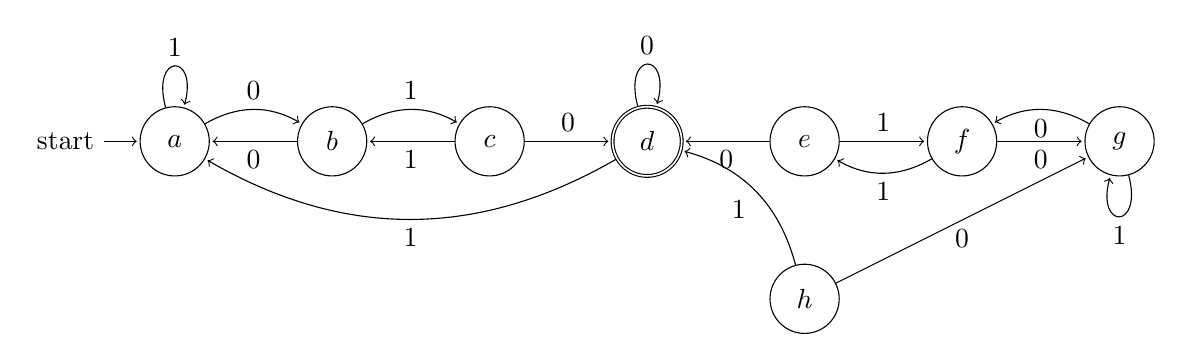
\begin{tikzpicture}[shorten >=1pt,node distance=2cm,on grid,auto]
  \node[state,initial] (a) {$a$};
  \node[state] (b) [right=of a] {$b$};
  \node[state] (c) [right=of b] {$c$};
  \node[state, accepting] (d) [right=of c] {$d$};
  \node[state] (e) [right=of d] {$e$};
  \node[state] (f) [right=of e] {$f$};
  \node[state] (g) [right=of f] {$g$};
  \node[state] (h) [below=of e] {$h$};

  \path[->]
    (a) edge [loop above] 	node {1} (a)
        edge [bend left] 	node {0} (b)
    (b) edge [bend left] 	node {1} (c)
        edge [below] 		node {0} (a)
    (c) edge [above] 		node {0} (d)
        edge [below] 		node {1} (b)
    (d) edge [loop above] 	node {0} (d)
        edge [bend left] 	node {1} (a)
    (e) edge 				node {0} (d)
        edge [above] 		node {1} (f)
    (f) edge [below]				node {0} (g)
        edge [bend left] 	node {1} (e)
    (g) edge [loop below] 	node {1} (g)
    	edge [bend right] 	node {0} (f)
    (h) edge [below]				node {0} (g)
        edge [bend right] 	node {1} (d);
\end{tikzpicture}

Jak widzimy $\textbf{M}$ to DFA. Naszym zdaniem będzie jego minimalizacja.


\subsection*{Minimalizacja DFA}
Algorytm minimalizacji DFA dzieli się na trzy etapy:
\begin{itemize}
    \item[1] Usuń z automatu wszystkie stany, które nie są osiągalne ze stanu początkowego.
    \item[2] Utwórz tabelę par stanów automatu$X_{i},X_{j}$, gdzie $X i \neq X j$.
    \subitem1 Zaznacz wszystkie pary stanów, gdzie $X_i \in F$ ($F$ - zbiór stanów akceptujących), a $X_j \notin F$.
    \subitem2 Dla każdej nie zaznaczonej jeszcze pary stanów oraz dla każdego elementu $a in A$ (A - skończony alfabet wejściowy) sprawdź, czy para $\lbrace\delta(X_i,a),\delta(X_j,a)\rbrace$ jest zaznaczona. Jeśli tak, zaznacz również $\lbrace X_i, X_j\rbrace$.
    \subitem3 Powtarzaj krok 2.2 tak długo, dopóki żadna zmiana w tabeli nie będzie już możliwa.
    \subitem4 Każda para, która pozostała niezaznaczona, zostaje stopiona do jednego stanu.
\end{itemize}
\subsection*{Rozwiązanie}
Już na pierwszy rzut oka widać, że wierzchołek \textbf{h} reprezentuje stan nieosiągalny (nie prowadzą do niego żadne strzałki). Usuwamy go.

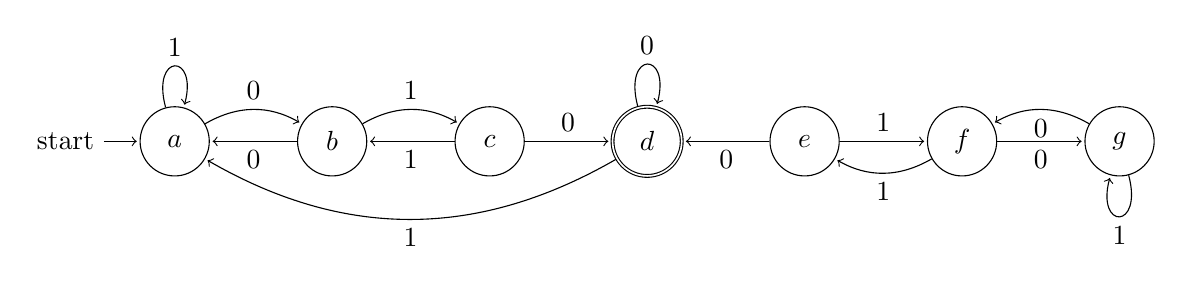
\begin{tikzpicture}[shorten >=1pt,node distance=2cm,on grid,auto]
  \node[state,initial] (a) {$a$};
  \node[state] (b) [right=of a] {$b$};
  \node[state] (c) [right=of b] {$c$};
  \node[state, accepting] (d) [right=of c] {$d$};
  \node[state] (e) [right=of d] {$e$};
  \node[state] (f) [right=of e] {$f$};
  \node[state] (g) [right=of f] {$g$};

  \path[->]
    (a) edge [loop above] 	node {1} (a)
        edge [bend left] 	node {0} (b)
    (b) edge [bend left] 	node {1} (c)
        edge [below] 		node {0} (a)
    (c) edge [above] 		node {0} (d)
        edge [below] 		node {1} (b)
    (d) edge [loop above] 	node {0} (d)
        edge [bend left] 	node {1} (a)
    (e) edge 				node {0} (d)
        edge [above] 		node {1} (f)
    (f) edge [below]				node {0} (g)
        edge [bend left] 	node {1} (e)
    (g) edge [loop below] 	node {1} (g)
    	edge [bend right] 	node {0} (f);
\end{tikzpicture}
Stanami nie osiągalnymi są też stany \textbf{e}, \textbf{f} oraz \textbf{g}. Nie da się do nich dostać startując ze stanu początkowego \textbf{a}. Usuwamy je.

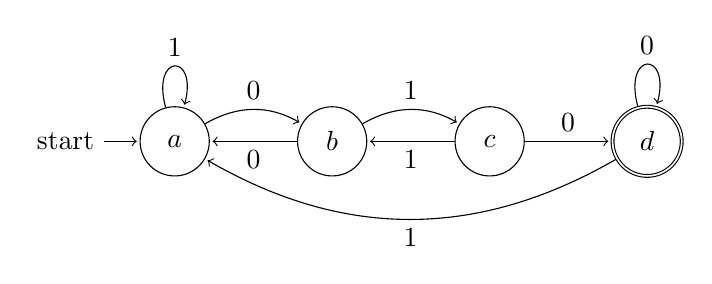
\begin{tikzpicture}[shorten >=1pt,node distance=2cm,on grid,auto]
  \node[state,initial] (a) {$a$};
  \node[state] (b) [right=of a] {$b$};
  \node[state] (c) [right=of b] {$c$};
  \node[state, accepting] (d) [right=of c] {$d$};

  \path[->]
    (a) edge [loop above] 	node {1} (a)
        edge [bend left] 	node {0} (b)
    (b) edge [bend left] 	node {1} (c)
        edge [below] 		node {0} (a)
    (c) edge [above] 		node {0} (d)
        edge [below] 		node {1} (b)
    (d) edge [loop above] 	node {0} (d)
        edge [bend left] 	node {1} (a);
\end{tikzpicture}\\
Następnym krokiem jest znalezienie stanów równoważnych. Tworzymy tabele.
\begin{table}[H]
    \centering
    \begin{tabular}{|c|c|c|c|c|}
    \hline
    		   & \textbf{a} & \textbf{b} & \textbf{c} & \textbf{d}\\\hline
    \textbf{a}\\\hline
    \textbf{b} & \\\hline
    \textbf{c} & &\\\hline
    \textbf{d} & X & X & X \\\hline
    \end{tabular}
    \label{tab:mytable}
\end{table}
Tylko \textbf{d} jest stanem końcowym, więc zaznaczamy cały ostatni rząd.
Przechodzimy do kroku 2.2. $\delta(b,0) = a$, $\delta(a,0) = b$. Para $[a,b]$ nie występuje na naszej tabeli. $\delta(b,1) = c$, $\delta(a,1) = a$. Ta para nie jest zaznaczona. $\delta(c,0) = d$, $\delta(a,0) = b$. Para $[d,b]$ jest zaznaczona, więc zaznaczamy parę $[c,a]$.
\begin{table}[H]
    \centering
    \begin{tabular}{|c|c|c|c|c|}
    \hline
    		   & \textbf{a} & \textbf{b} & \textbf{c} & \textbf{d}\\\hline
    \textbf{a}\\\hline
    \textbf{b} & \\\hline
    \textbf{c} & X & \\\hline
    \textbf{d} & X & X & X \\\hline
    \end{tabular}
    \label{tab:mytable}
\end{table}
$\delta(c,0) = d$, $\delta(b,0) = a$. Zaznaczamy $[c,b]$. (Pomijam sprawdzanie kolejnych $a$, ponieważ osiągnęliśmy już stan akceptujący. 
\begin{table}[H]
    \centering
    \begin{tabular}{|c|c|c|c|c|}
    \hline
    		   & \textbf{a} & \textbf{b} & \textbf{c} & \textbf{d}\\\hline
    \textbf{a}\\\hline
    \textbf{b} & \\\hline
    \textbf{c} & X & \\\hline
    \textbf{d} & X & X & X \\\hline
    \end{tabular}
    \label{tab:mytable}
\end{table}
Wróćmy teraz do stanu $[b,a]$. Zaznaczyliśmy $[c,a]$, więc musimy także zaznaczyć $[b,a]$, ponieważ $\delta(b,1) = c$ $\delta(a,1) = a$, to nasz stan akceptujący.
\begin{table}[H]
    \centering
    \begin{tabular}{|c|c|c|c|c|}
    \hline
    		   & \textbf{a} & \textbf{b} & \textbf{c} & \textbf{d}\\\hline
    \textbf{a}\\\hline
    \textbf{b} & X\\\hline
    \textbf{c} & X & X\\\hline
    \textbf{d} & X & X & X \\\hline
    \end{tabular}
    \label{tab:mytable}
\end{table}
Jak wynika z opisu algorytmu oraz powyższej tabeli w naszym automacie nie ma par stanów, które można by było scalić. Znaczy to, że automat otrzymany przez nas jest automatem minimalnym.\\
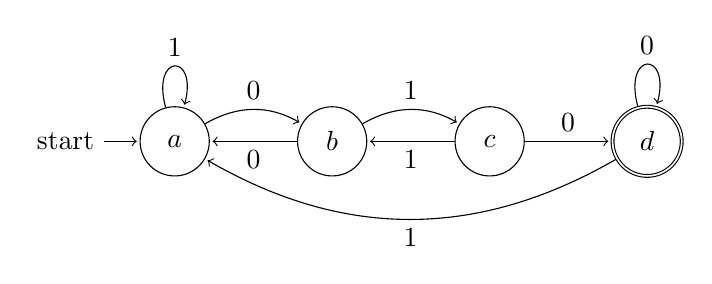
\begin{tikzpicture}[shorten >=1pt,node distance=2cm,on grid,auto]
  \node[state,initial] (a) {$a$};
  \node[state] (b) [right=of a] {$b$};
  \node[state] (c) [right=of b] {$c$};
  \node[state, accepting] (d) [right=of c] {$d$};

  \path[->]
    (a) edge [loop above] 	node {1} (a)
        edge [bend left] 	node {0} (b)
    (b) edge [bend left] 	node {1} (c)
        edge [below] 		node {0} (a)
    (c) edge [above] 		node {0} (d)
        edge [below] 		node {1} (b)
    (d) edge [loop above] 	node {0} (d)
        edge [bend left] 	node {1} (a);
\end{tikzpicture}
\end{document}